\documentclass[tikz,convert={outfile=\jobname.png}]{standalone}
\begin{document}
    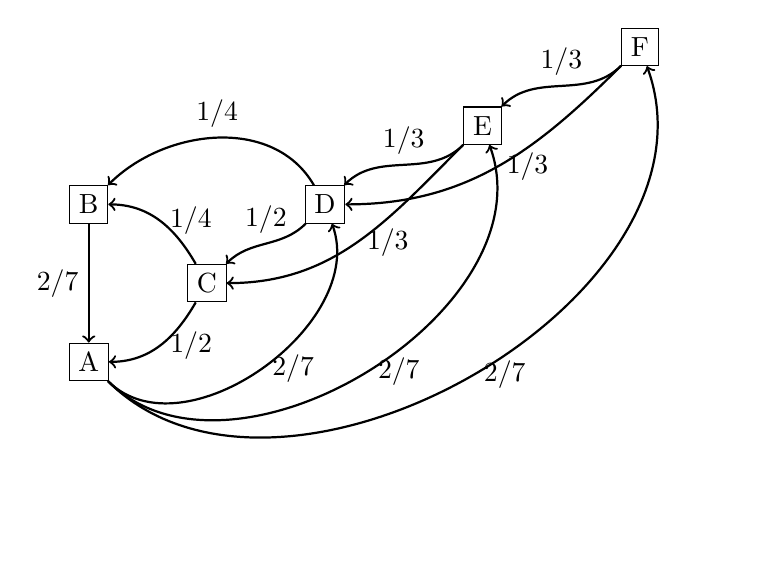
\begin{tikzpicture}
        \node [draw] (A) at (0, 0) {A};
        \node [draw] (B) at (0, 2) {B};
        \node [draw] (C) at (1.5, 1) {C};
        \node [draw] (D) at (3, 2) {D};
        \node [draw] (E) at (5, 3) {E};
        \node [draw] (F) at (7, 4) {F};

        \draw (A) edge[out=-45, in=-70, ->, thick] node [right] {$2/7$} (F);
        \draw (A) edge[out=-45, in=-70, ->, thick] node [right] {$2/7$} (E);
        \draw (A) edge[out=-45, in=-70, ->, thick] node [right] {$2/7$} (D);

        \draw (B) edge[out=-90, in=90, ->, thick] node [left] {$2/7$} (A);

        \draw (C) edge[out=-120, in=0, ->, thick] node [right] {$1/2$} (A);
        \draw (C) edge[out=120, in=0, ->, thick] node [right] {$1/4$} (B);

        \draw (D) edge[out=120, in=45, ->, thick] node [above] {$1/4$} (B);
        \draw (D) edge[out=-135, in=45, ->, thick] node [above] {$1/2$} (C);

        \draw (E) edge[out=-135, in=0, ->, thick] node [right] {$1/3$} (C);
        \draw (E) edge[out=-135, in=45, ->, thick] node [above] {$1/3$} (D);

        \draw (F) edge[out=-135, in=0, ->, thick] node [right] {$1/3$} (D);
        \draw (F) edge[out=-135, in=45, ->, thick] node [above] {$1/3$} (E);

    \end{tikzpicture}
\end{document}
